\chapter{Odometria}
	La soluzione utilizzata per rilevare la posizione dei robot all'interno dell'arena include l'utilizzo di metodi di computer vision in grado di rilevare contemporaneamente sia la posizione che l'orientamento di marker grafici attraverso le immagini fornite dalla webcam.
	
	L'acquisizione delle immagini dalla fotocamera avviene tramite il nodo ROS \emph{usb\_cam} che comunica con il sensore di immagini utilizzando il protocollo V4L (video for linux) e pubblica i fotogrammi ottenuti tramite \emph{image\_transport}, il protocollo standard per la trasmissione delle immagini in ROS.

\section{Calibrazione della fotocamera}
	Per riconoscere in maniera ottimale i marker l'immagine proveniente dalla fotocamera deve essere rettificata per bilanciare la distorsione introdotta dalle lenti.
	
	Per ottenere una rettificazione ottimale \`e necessario generare il file di calibrazione della fotocamera, questo file \`e ottenuto utilizzando l'applicazione ROS \emph{camera\_calibration} che calcola i parametri di distorsione.
	
	La procedura di calibrazione implica l'utilizzo di una scacchiera con dimensioni ben definite
	\begin{figure}[H]
	\centering
	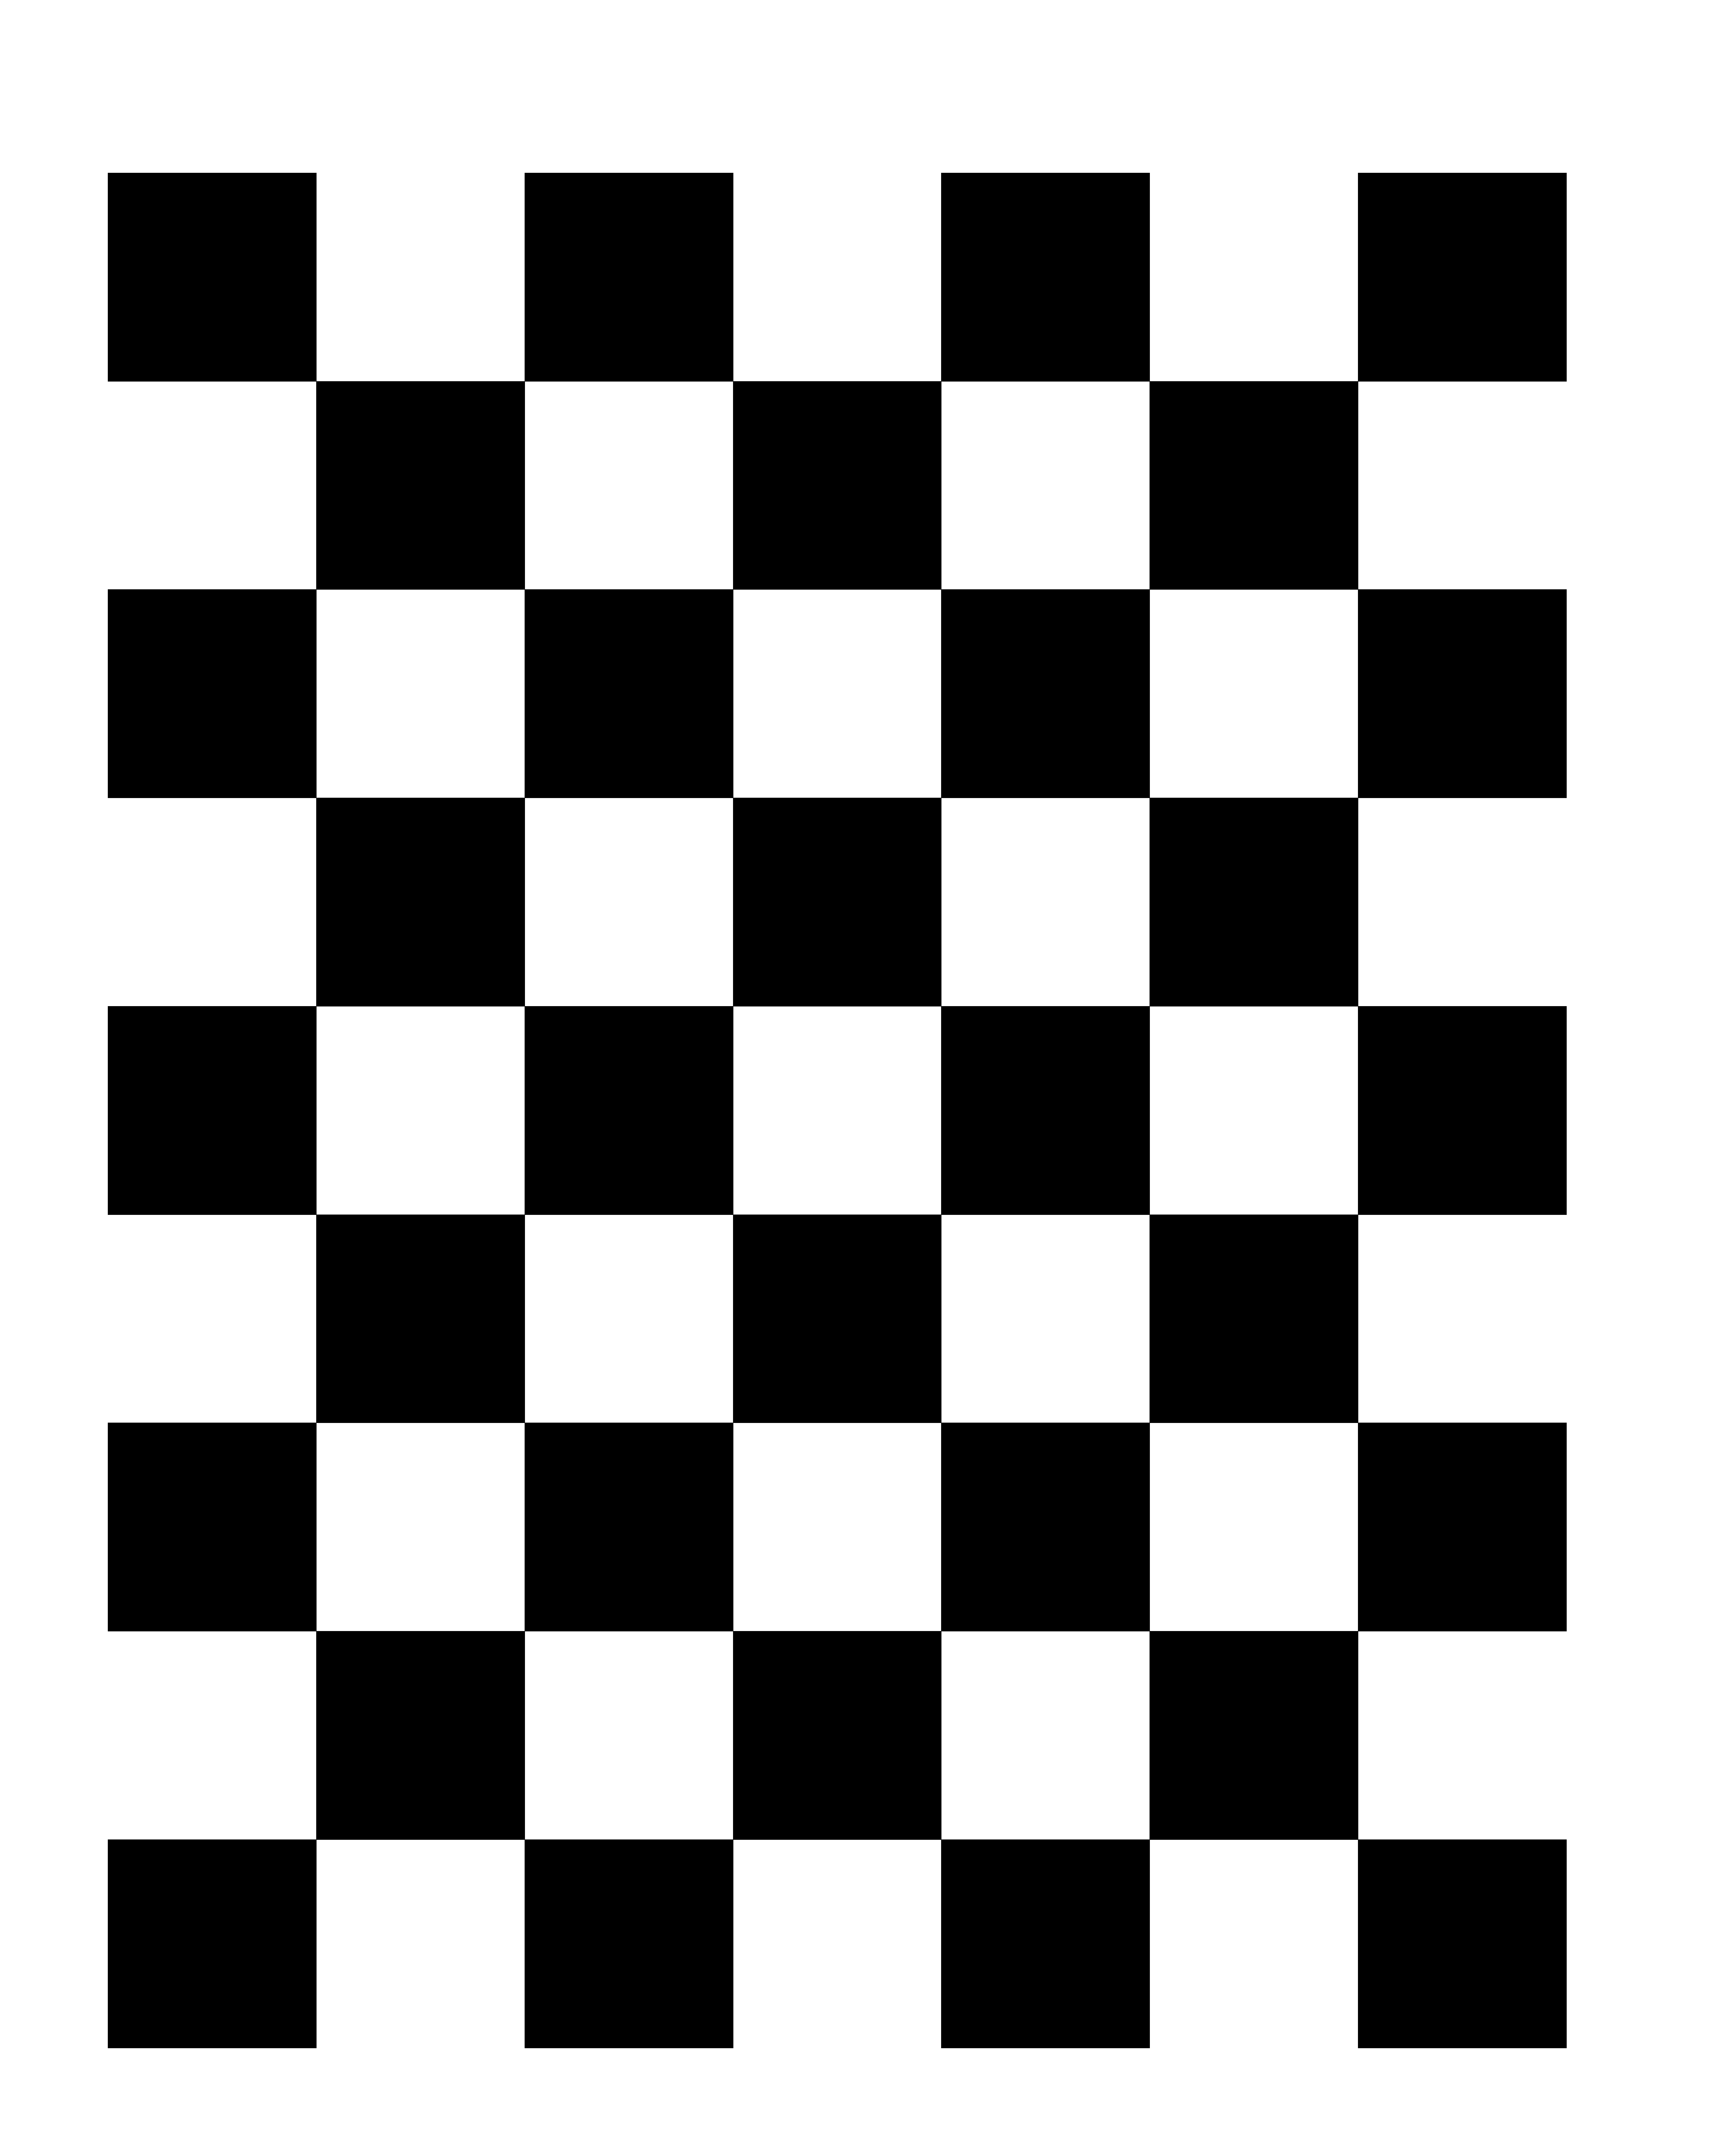
\includegraphics[width=0.4\linewidth, angle=90]{./images/check-108}
	\caption{Scacchiera 8 x 6}
	\label{fig:check-108}
	\end{figure}

	Una volta avviata l'applicazione si procede all'acquisizione dei dati traslando e ruotando la scacchiera lungo l'intero campo visivo della fotocamera fino a quando il software non comunica di aver acquisito sufficienti informazioni per la calibrazione. Il software ora pu\`o calcolare i dati di calibrazione e salvarli in un file formato YAML.
	
	La vera rettificazione dell'immagine avviene attraverso il nodo \emph{image\_proc} che processa l'immagine utilizzando i dati di calibrazione e restituisce l'immagine rettificata sempre utilizzando il protocollo di trasmissione di immagini di ROS.
	\huge
	 \emph{inserire immagini di esempio immagini rettificate e non}
	 \normalsize
	 
\section{Software di riconoscimento: ArUco}
	
\subsection{Markers}
\subsection{Boards}
\section{Compatibilit\`a con ROS}
\subsection{TF}